%! TEX root = ../main.tex
% ==============================================================
% IMMUTABLE — generated automatically, do not edit this block
%
% — Provenance ───────────────────────────────────────────────────
%   script            : plotter.py::plot_wind_snr
%   computed_in       : 
%   plot_type         : wind_snr
%   data_class        : 
%   generated_at      : 2026-04-24T15:45:42
%   findings_doc      : 
%
% — Thesis context ──────────────────────────────────────────────
%   chapter           : 04
%   caption_label     : fig:ch04_wind_snr
%   caption_short     : Spectral SNR per probe: ratio of paddle-frequency FFT amplitude to wind-noise amplitude integrated over the 0.1\,Hz FFT window at each paddle frequency (512 wave runs; wind-noise baseline from 18 f…
%
% — Filters ────────────────────────────────────────────────────
%   panel             : 
%   wind              : 
%   amplitude [V]     : 
%   frequency [Hz]    : 
%   probes            : 9373/170, 12400/250, 9373/340, 8804/250
%   run_category      : 
%   quality_flag      : 
%   mooring           : 
%
% — Data provenance ────────────────────────────────────────────
%   n_runs            : 637
%   in_probes_used    : 9373/170+9373/340, 9373/250
%   out_probes_used   : 11800/250, 12400/170+12400/340, 12400/250
%   probe_configs     : initial_setup, march2026_better_rearranging, march2026_rearranging, nov_normalt_oppsett
%   non_final_config_n: 169
%   datasets        :
%     PROCESSED-20260326-ProbePos4_31_FPV_2-tett6roof-under9Mooring-height100-lowrange
%     PROCESSED-20260327-ProbePos4_31_FPV_2-tett6roof-under9Mooring30-height100-lowrange
%   run_paths       :
%     (omitted — aggregate over > threshold runs, see datasets)
%
% — Method / numerical parameters ─────────────────────────────
%   grouper           : 
%   collapse_panels   : 
%   fft_window_hz     : 
%   extra_params      : 
%
% — Summary stats cited in caption ────────────────────────────
%   (none registered — pass extra_stats=... to build_fig_meta)
%
% — Subfigures available ───────────────────────────────────────
%     FIGURES/ch04_wind_snr.pdf
% ── end immutable block ─────────────────────────────────────────
\begin{figure}[htbp]
  \centering
  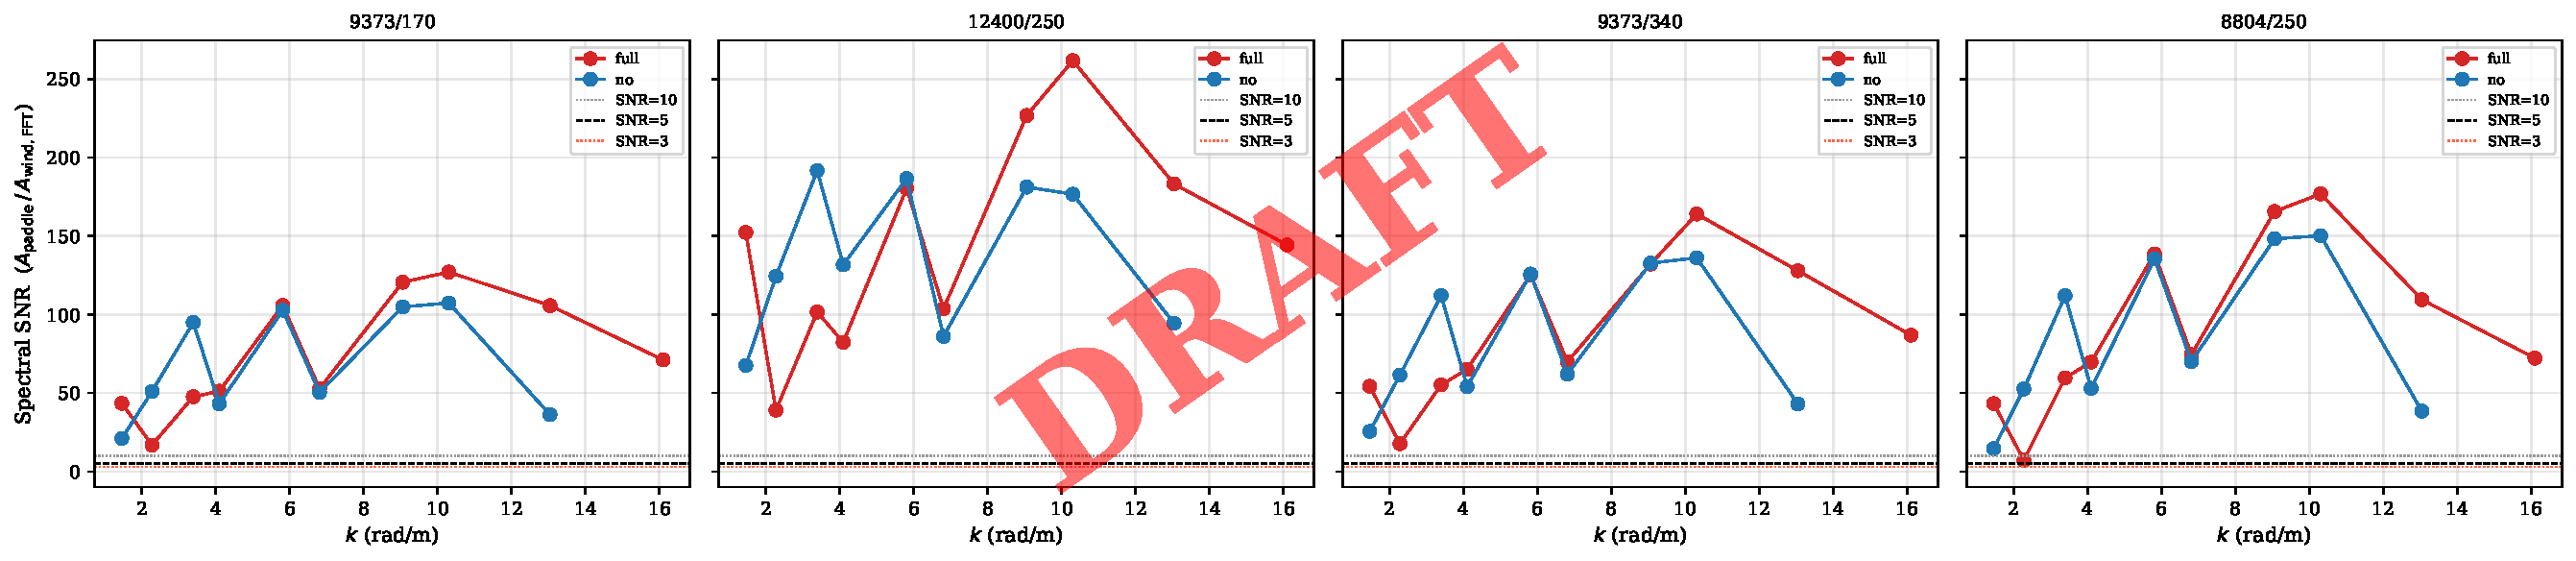
\includegraphics[width=\linewidth]{FIGURES/ch04_wind_snr.pdf}
  \caption[Spectral SNR per probe: ratio of paddle-frequency FFT amplitude to wind-noise amplitude integrated over the 0]{
    Spectral SNR per probe: ratio of paddle-frequency FFT amplitude to wind-noise amplitude integrated over the 0.1\,Hz FFT window at each paddle frequency (512 wave runs; wind-noise baseline from 18 full-wind no-wave runs). Horizontal lines: SNR~=~10 (dotted grey), 5 (dashed black), 3 (dotted red, critical). SNR~$<$~3 indicates wind dominates the FFT measurement.
  }
  \label{fig:ch04_wind_snr}
\end{figure}
